\documentclass{beamer}

\usepackage{amsmath}

\usetheme{AnnArbor}
\usecolortheme{crane}
\usefonttheme[onlymath]{serif}

\title{Deep Learning - Foundations and Concepts}
\subtitle{Chapter 2. Probabilities}
\author{nonlineark@github}
\date{\today}

\begin{document}

\begin{frame}
    \titlepage
\end{frame}

\begin{frame}
    \frametitle{Outline}
    \tableofcontents
\end{frame}

\section{The Rules of Probability}

\begin{frame}
    \frametitle{The sum and product rules}
    \begin{itemize}
        \item Sum rule: $p(X)=\sum_{Y}p(X,Y)$.
        \item Product rule: $p(X,Y)=p(Y|X)p(X)$.
    \end{itemize}
\end{frame}

\begin{frame}
    \frametitle{Bayes' theorem}
    \begin{itemize}
        \item Bayes' theorem:
        \begin{align*}
            p(Y|X)&=\frac{p(X|Y)p(Y)}{p(X)} \\
            &=\frac{p(X|Y)p(Y)}{\sum_{Y}p(X|Y)p(Y)}
        \end{align*}
        \item Prior and posterior probabilities:
        \begin{itemize}
            \item $p(Y)$ is the prior probability, because it is available \emph{before} we observe the event $X$.
            \item $p(Y|X)$ is the posterior probability, because it is obtained \emph{after} we have observed the event $X$.
        \end{itemize}
    \end{itemize}
\end{frame}

\section{Probability Densities}

\begin{frame}
    \frametitle{Probability densities}
    \begin{itemize}
        \item A probability density $p(x)$ is a real function satisfies the following two conditions\footnotemark:
        \begin{itemize}
            \item $p(x)\ge{}0$.
            \item $\int_{-\infty}^{+\infty}p(x)\mathrm{d}x=1$.
        \end{itemize}
        \item The \emph{cumulative distribution function} is given by $P(x)=\int_{-\infty}^{x}p(t)\mathrm{d}t$, and usually we have $P'(x)=p(x)$.
        \item These definitions can easily be extended to higher dimensions.
    \end{itemize}
    \footnotetext{This is \emph{not} a mathematically robust definition, but it suffices for this course.}
\end{frame}

\begin{frame}
    \frametitle{Probability densities}
    \begin{itemize}
        \item Sum rule: $p(x)=\int{}p(x,y)\mathrm{d}y$.
        \item Product rule: $p(x,y)=p(y|x)p(x)$.
        \item Bayes' theorem: $p(y|x)=\frac{p(x|y)p(y)}{p(x)}=\frac{p(x|y)p(y)}{\int{}p(x|y)p(y)\mathrm{d}y}$.
    \end{itemize}
\end{frame}

\begin{frame}
    \frametitle{Expectations and covariances}
    \begin{itemize}
        \item Expectation of $f$:
        \begin{itemize}
            \item Discrete case: $E(f)=\sum_{x}p(x)f(x)$.
            \item Continuous case: $E(f)=\int{}p(x)f(x)\mathrm{d}x$.
        \end{itemize}
        \item Variance of $f$: $\mathrm{var}(f)=E((f(x)-E(f))^{2})=E(f^{2})-E(f)^{2}$.
        \item Covariance of:
        \begin{itemize}
            \item Two random variables: $\mathrm{cov}(x,y)=E((x-E(x))(y-E(y)))=E(xy)-E(x)E(y)$.
            \item Two vectors: $\mathrm{cov}(x,y)=E((x-E(x))(y-E(y))^{T})=E(xy^{T})-E(x)E(y^{T})$.
        \end{itemize}
    \end{itemize}
\end{frame}

\begin{frame}
    \frametitle{Example distributions}
    \begin{itemize}
        \item Uniform distribution: $p(x)=\frac{1}{d-c},\quad{}x\in(c,d)$.
        \item Exponential distribution: $p(x;\lambda)=\lambda\exp(-\lambda{}x)$.
        \item Laplace distribution: $p(x;\mu,\gamma)=\frac{1}{2\gamma}\exp(-\frac{|x-\mu|}{\gamma})$.
        \item Dirac delta function: $p(x;\mu_{1},\hdots,\mu_{N})=\frac{1}{N}\sum_{n=1}^{N}\delta(x-\mu_{n})$.
    \end{itemize}
\end{frame}

\section{The Gaussian Distribution}

\begin{frame}
    \frametitle{The Gaussian distribution}
    \begin{itemize}
        \item Definition: $\mathcal{N}(x;\mu,\sigma^{2})=\frac{1}{\sqrt{2\pi\sigma^{2}}}\exp(-\frac{(x-\mu)^{2}}{2\sigma^{2}})$.
        \item Mean: $E(x)=\int_{-\infty}^{+\infty}\mathcal{N}(x;\mu,\sigma^{2})x\mathrm{d}x=\mu$.
        \item Variance: $\mathrm{var}(x)=E(x^{2})-E(x)^{2}=\sigma^{2}$.
    \end{itemize}
\end{frame}

\begin{frame}
    \frametitle{Maximum likelihood and its bias}
    \begin{block}{Problem}
        We have $N$ observations of a random variable $x$: $x_{1},\hdots,x_{N}$ that are drawn independently from a Gaussian distribution whose mean $\mu$ and variance $\sigma^{2}$ are unknown. How do we determine these parameters from the data set?
    \end{block}
\end{frame}

\begin{frame}
    \frametitle{Maximum likelihood and its bias}
    \begin{block}{Problem'}
        Find $\mu$ and $\sigma^{2}$ such that the probability of the data set
        \begin{equation*}
            p(x_{1},\hdots,x_{N};\mu,\sigma^{2})=\prod_{n=1}^{N}\mathcal{N}(x_{n};\mu,\sigma^{2})
        \end{equation*}
        is maximized.
    \end{block}
\end{frame}

\begin{frame}
    \frametitle{Maximum likelihood and its bias}
    \begin{block}{Problem''}
        Let's minimize
        \begin{align*}
            L&=-\log{}p(x_{1},\hdots,x_{N};\mu,\sigma^{2}) \\
            &=\frac{1}{2\sigma^{2}}\sum_{n=1}^{N}(x_{n}-\mu)^{2}+\frac{N}{2}\log\sigma^{2}+\frac{N}{2}\log(2\pi)
        \end{align*}
        instead.
    \end{block}
\end{frame}

\begin{frame}
    \frametitle{Maximum likelihood and its bias}
    \begin{align*}
        \frac{\partial{}L}{\partial\mu}&=\frac{1}{\sigma^{2}}\sum_{n=1}^{N}(\mu-x_{n})=\frac{N}{\sigma^{2}}(\mu-\frac{1}{N}\sum_{n=1}^{N}x_{n}) \\
        \frac{\partial{}L}{\partial\sigma}&=\frac{N}{\sigma^{3}}(\sigma^{2}-\frac{1}{N}\sum_{n=1}^{N}(x_{n}-\mu)^{2})
    \end{align*}
    Setting $\frac{\partial{}L}{\partial\mu}$ and $\frac{\partial{}L}{\partial\sigma}$ to $0$, we have:
    \begin{align*}
        \mu_{ML}&=\frac{1}{N}\sum_{n=1}^{N}x_{n} \\
        \sigma^{2}_{ML}&=\frac{1}{N}\sum_{n=1}^{N}(x_{n}-\mu_{ML})^{2}
    \end{align*}
\end{frame}

\begin{frame}
    \frametitle{Maximum likelihood and its bias}
    Let's do some sanity check. Suppose that $x_{1},\hdots,x_{N}$ are generated from a Gaussian distribution whose true parameters are $\mu$ and $\sigma^{2}$. We expect the calculated parameters $\mu_{ML}$ and $\sigma^{2}_{ML}$ to be equal to $\mu$ and $\sigma^{2}$
    respectively. Or put another way, we expect:
    \begin{align*}
        E(\mu_{ML})&=\mu \\
        E(\sigma^{2}_{ML})&=\sigma^{2}
    \end{align*}
    Is that true?
\end{frame}

\begin{frame}
    \frametitle{Maximum likelihood and its bias}
    \begin{align*}
        E(\mu_{ML})&=E(\frac{1}{N}\sum_{n=1}^{N}x_{n})=\frac{1}{N}\sum_{n=1}^{N}E(x_{n})=\mu \\
        E(\mu_{ML}^{2})&=E((\frac{1}{N}\sum_{n=1}^{N}x_{n})^{2}) \\
        &=\frac{1}{N^{2}}(\sum_{1\le{}m\ne{}n\le{}N}E(x_{m}x_{n})+\sum_{n=1}^{N}E(x_{n}^{2}))=\mu^{2}+\frac{1}{N}\sigma^{2} \\
        E(\sigma^{2}_{ML})&=E(\frac{1}{N}\sum_{n=1}^{N}(x_{n}-\mu_{ML})^{2}) \\
        &=\frac{1}{N}\sum_{n=1}^{N}E(x_{n}^{2})-E(\mu_{ML}^{2})=\frac{N-1}{N}\sigma^{2}
    \end{align*}
\end{frame}

\begin{frame}
    \frametitle{Maximum likelihood and its bias}
    For a Gaussian distribution, the following estimate for the variance parameter is unbiased:
    \begin{equation*}
        \tilde{\sigma}^{2}=\frac{N}{N-1}\sigma^{2}_{ML}=\frac{1}{N-1}\sum_{n=1}^{N}(x_{n}-\mu_{ML})^{2}
    \end{equation*}
\end{frame}

\begin{frame}
    \frametitle{Linear regression from a maximum likelihood perspective}
    \begin{block}{Problem}
        Assume that given the value of $x_{n}$, the corresponding value of $t_{n}$ has a Gaussian distribution with a mean equal to the value $y(x_{n};w)$ and a variance $\sigma^{2}$ (where the parameters $w$ and $\sigma^{2}$ are to be determined). Maximize the
        likelihood function:
        \begin{equation*}
            p(t|x;w,\sigma^{2})=\prod_{n=1}^{N}\mathcal{N}(t_{n};y(x_{n};w),\sigma^{2})
        \end{equation*}
    \end{block}
\end{frame}

\begin{frame}
    \frametitle{Linear regression from a maximum likelihood perspective}
    Again, we minimize the negative log function:
    \begin{align*}
        L&=-\log{}p(t|x;w,\sigma^{2}) \\
        &=\frac{1}{2\sigma^{2}}\sum_{n=1}^{N}(y(x_{n};w)-t_{n})^{2}+\frac{N}{2}\log\sigma^{2}+\frac{N}{2}\log(2\pi)
    \end{align*}
    We see that maximizing the likelihood function for $w$ is equivalent to minimizing the error function defined by:
    \begin{equation*}
        E(w)=\frac{1}{2}\sum_{n=1}^{N}(y(x_{n};w)-t_{n})^{2}
    \end{equation*}
\end{frame}

\begin{frame}
    \frametitle{Linear regression from a maximum likelihood perspective}
    What has us gained from looking at the linear regression problem from a maximum likelihood perspective? Instead of a point estimate, we now have a predictive distribution:
    \begin{equation*}
        p(\hat{t}|\hat{x};w_{ML},\sigma^{2}_{ML})=\mathcal{N}(\hat{t};y(\hat{x};w_{ML}),\sigma^{2}_{ML})
    \end{equation*}
    where
    \begin{align*}
        w_{ML}&=(XX^{T})^{-1}Xt \\
        \sigma^{2}_{ML}&=\frac{1}{N}\sum_{n=1}^{N}(y(x_{n};w_{ML})-t_{n})^{2}
    \end{align*}
\end{frame}

\section{Transformation of Densities}

\begin{frame}
    \frametitle{Probability densities are integrand}
    When changing variable, we need to be aware that probability densities are integrand:
    \begin{equation*}
        p(x)\mathrm{d}x=p(g(y))\mathrm{d}g(y)=p(g(y))g'(y)\mathrm{d}y
    \end{equation*}
    For multivariate case:
    \begin{equation*}
        p(x)\mathrm{d}x=p(g(y))\det\frac{\partial(x_{1},\hdots,x_{N})}{\partial(y_{1},\hdots,y_{N})}\mathrm{d}y
    \end{equation*}
\end{frame}

\begin{frame}
    \frametitle{Transformation of densities}
    Consider the problem of finding the maximum for a probability density $p(x)$. Say the maximum happens when $x=\hat{x}$. Now we do a change of variable $x=g(y)$, does the maximum for the new probability density happens at $\hat{y}$ where $\hat{x}=g(\hat{y})$?
    \begin{align*}
        q(y)&=p(g(y))g'(y) \\
        q'(y)&=p'(g(y))(g'(y))^{2}+p(g(y))g''(y)
    \end{align*}
    We see that this is usually not the case, unless $g$ is a linear transformation.
\end{frame}

\begin{frame}
    \frametitle{Transformation of densities}
    \begin{figure}
        \caption{Transformation of the mode of a density}
        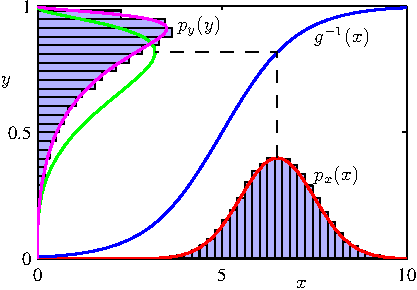
\includegraphics{Figure_12.pdf}
    \end{figure}
\end{frame}

\section{Information Theory}

\begin{frame}
    \frametitle{Information}
    Intuitively, if we have two events $x$ and $y$ that are unrelated, the information gained from observing both of them should be the sum of the information gained from each of them separately:
    \begin{align*}
        h(x,y)&=h(x)+h(y) \\
        p(x,y)&=p(x)p(y)
    \end{align*}
    From this it's plausible to define $h(x)=-\log_{2}p(x)$.
\end{frame}

\begin{frame}
    \frametitle{Entropy}
    The entropy of a random variable $x$ is defined as the expectation of the information $h(x)$ with respect to the distribution $p(x)$:
    \begin{equation*}
        H[x]=E(h)=\sum_{x}p(x)h(x)=-\sum_{x}p(x)\log_{2}p(x)
    \end{equation*}
    When using logarithms to the base of $2$, the units of $H[x]$ are bits. From now on, we will switch to the use of natural logarithms in defining entropy, which is measured in units of \emph{nats}.
\end{frame}

\begin{frame}
    \frametitle{Maximum entropy for the discrete case}
    Let $H(p)=-\sum_{n=1}^{N}p_{i}\log{}p_{i}$, where $0\le{}p_i\le{}1$, it's easy to see that $H(p)$ achieves its minimum $0$ for unit vectors. When does $H(p)$ achieves its maximum?
\end{frame}

\begin{frame}
    \frametitle{Maximum entropy for the discrete case}
    Finding the maximum of $H(p)$ under the constraint $g(p)=\sum_{n=1}^{N}p_{n}-1=0$ using Lagrange multiplier:
    \begin{align*}
        \nabla{}H(p)&=\lambda\nabla{}g(p) \\
        -(\log{}p_{n}+1)&=\lambda \\
        p_{n}&=\frac{1}{N} \\
        \max{}H(p)&=\log{}N
    \end{align*}
\end{frame}

\begin{frame}
    \frametitle{Differential entropy and its maximum}
    For the continuous case, we define the differential entropy to be:
    \begin{equation*}
        H[x]=-\int{}p(x)\log{}p(x)\mathrm{d}x
    \end{equation*}
\end{frame}

\begin{frame}
    \frametitle{Differential entropy and its maximum}
    Finding the maximum of $H(p)$ under the following constraints:
    \begin{align*}
        \int_{-\infty}^{+\infty}p(x)\mathrm{d}x&=1 \\
        \int_{-\infty}^{+\infty}xp(x)\mathrm{d}x&=\mu \\
        \int_{-\infty}^{+\infty}(x-\mu)^{2}p(x)\mathrm{d}x&=\sigma^{2}
    \end{align*}
    The maximum happens when $p(x)$ is the Gaussian distribution:
    \begin{equation*}
        p(x)=\frac{1}{\sqrt{2\pi\sigma^{2}}}\exp(-\frac{(x-\mu)^{2}}{2\sigma^{2}})
    \end{equation*}
    and
    \begin{equation*}
        \max{}H(p)=\frac{1}{2}(1+\log(2\pi\sigma^{2}))
    \end{equation*}
\end{frame}

\begin{frame}
    \frametitle{Kullback-Leibler divergence}
    \begin{block}{Problem}
        Consider some unknown distribution $p(x)$. Suppose we have modelled $p(x)$ using an approximating distribution $q(x)$. If we use $q(x)$ to construct a coding scheme, what is the average additional amount of information required?
    \end{block}
\end{frame}

\begin{frame}
    \frametitle{Kullback-Leibler divergence}
    \begin{align*}
        KL(p||q)&=-\int{}p(x)\log{}q(x)\mathrm{d}x-(-\int{}p(x)\log{}p(x)\mathrm{d}x) \\
        &=-\int{}p(x)\log\frac{q(x)}{p(x)}\mathrm{d}x
    \end{align*}
    This is also known as the relative entropy or Kullback-Leibler divergence, or KL divergence, between the distributions $p(x)$ and $q(x)$.
\end{frame}

\begin{frame}
    \frametitle{Kullback-Leibler divergence}
    If $f$ is a convex function, then Jensen's inequality holds:
    \begin{align*}
        f(E(x))&\le{}E(f) \\
        f(\sum_{n=1}^{N}p_{n}x_{n})&\le\sum_{n=1}^{N}p_{n}f(x_{n}) \\
        f(\int{}xp(x)\mathrm{d}x)&\le\int{}p(x)f(x)\mathrm{d}x
    \end{align*}
    Notice that $-\log{}x$ is a convex function, we have:
    \begin{equation*}
        KL(p||q)=\int{}p(x)(-\log\frac{q(x)}{p(x)})\mathrm{d}x\ge-\log\int{}p(x)\frac{q(x)}{p(x)}\mathrm{d}x=0
    \end{equation*}
    The equality will hold iff. $q=p$.
\end{frame}

\begin{frame}
    \frametitle{Kullback-Leibler divergence}
    Minimizing the Kullback-Leibler divergence is equivalent to maximizing the likelihood function:
    \begin{equation*}
        KL(p||q)\approx\frac{1}{N}\sum_{n=1}^{N}(-\log{}q(x_{n};\theta)+\log{}p(x_{n}))
    \end{equation*}
    The first term is the negative $\log$ likelihood function for $\theta$ under the distribution $q(x;\theta)$ evaluated using the training set.
\end{frame}

\begin{frame}
    \frametitle{Conditional entropy}
    On average, if value for one random variable is already known, what is the additional information needed to specify value for another random variable?
    \begin{align*}
        H[y|x]&=-\iint{}p(x,y)\log{}p(y|x)\mathrm{d}x\mathrm{d}y \\
        H[x,y]&=H[y|x]+H[x]
    \end{align*}
\end{frame}

\begin{frame}
    \frametitle{Mutual information}
    For two random variables, are they "close" to being indepedent?
    \begin{align*}
        I[x,y]&=KL(p(x,y)||p(x)p(y)) \\
        &=-\iint{}p(x,y)\log\frac{p(x)p(y)}{p(x,y)}\mathrm{d}x\mathrm{d}y
    \end{align*}
    It's easy to see that:
    \begin{equation*}
        I[x,y]=H[x]-H[x|y]=H[y]-H[y|x]
    \end{equation*}
\end{frame}

\section{Bayesian Probabilities}

\begin{frame}
    \frametitle{Model parameters}
    Denote the training data set by $\mathcal{D}$, and the parameters in the model by $w$.
    \begin{itemize}
        \item $p(w)$ is our assumptions about $w$ before observing $\mathcal{D}$.
        \item $p(\mathcal{D}|w)$ is the likelihood function.
        \item $p(w|\mathcal{D})$ is the uncertainty in $w$ after we have observed $\mathcal{D}$.
    \end{itemize}
    We have:
    \begin{align*}
        p(w|\mathcal{D})&=\frac{p(\mathcal{D}|w)p(w)}{p(\mathcal{D})} \\
        &=\frac{p(\mathcal{D}|w)p(w)}{\int{}p(\mathcal{D}|w)p(w)\mathrm{d}w}
    \end{align*}
\end{frame}

\begin{frame}
    \frametitle{Regularization}
    When choosing the model parameters $w$, instead of maximizing the likelihood function $p(\mathcal{D}|w)$, we maximize the posterior probability $p(w|\mathcal{D})$:
    \begin{equation*}
        -\log{}p(w|\mathcal{D})=-\log{}p(\mathcal{D}|w)-\log{}p(w)+\log{}p(\mathcal{D})
    \end{equation*}
    Say each $w_{m}$ conforms to a Gaussian distribution:
    \begin{equation*}
        p(w)=p(w;\sigma^{2})=\prod_{m=0}^{M}\mathcal{N}(w_{m};0,\sigma^{2})
    \end{equation*}
    Then we have:
    \begin{equation*}
        -\log{}p(w|\mathcal{D})=-\log{}p(\mathcal{D}|w)+\frac{1}{2\sigma^{2}}\sum_{m=0}^{M}w_{m}^{2}+\mathrm{const}
    \end{equation*}
    The second term on the right hand side is indeed the penalty term.
\end{frame}

\begin{frame}
    \frametitle{Bayesian machine learning}
    If we are interested in the distribution of $t$ given both $x$ and $\mathcal{D}$, taking into consideration the uncertainty in the value of $w$, we have the fully Bayesian treatment:
    \begin{equation*}
        p(t|x,\mathcal{D})=\int{}p(t|x,w)p(w|\mathcal{D})\mathrm{d}w
    \end{equation*}
    \begin{itemize}
        \item The fully Bayesian treatment averages over all possible models:
        \begin{itemize}
            \item Less likely to lead to over-fitting.
            \item Prefer models of intermediate complexity.
        \end{itemize}
        \item Integrating over the space of parameters is typically infeasible.
    \end{itemize}
\end{frame}

\end{document}